\PassOptionsToPackage{x11names}{xcolor}
\documentclass[tikz, margin=5pt]{standalone}
\usepackage{amsmath}

%% use article
%\documentclass[landscape]{article}
%\usepackage[scale=0.8]{geometry}
%\usepackage[x11names]{xcolor}
%\usepackage{tikz}

\usetikzlibrary{
  arrows.meta,
  chains,
  matrix,
  positioning,
}

\makeatletter
\def\@currentColor{white}

\tikzset{
  set color/.code = { \gdef\@currentColor{#1} },
  lower box/.style = {
    draw,
    fill=\@currentColor,
    minimum height=2.5em,
    inner xsep=2pt,
    font=\color{white}\ttfamily
  },
  matrix default/.style = {
    matrix of math nodes
  },
  upper matrix/.style = {
    matrix default,
    column sep=0pt,
    below delimiter=\}
    %set color=Green3, % set default color before key "lower box" is passed
    %nodes=lower box
  },
  lower matrix/.style = {
    matrix default,
    row sep=0pt,
    %column sep=0pt,
    %set color=Green3, % set default color before key "lower box" is passed
    %nodes=lower box
  },
}
%\tikzset{
  %set color/.code = { \gdef\@currentColor{#1} },
  %%% node
  %box/.style = {
    %draw,
    %rounded corners=2mm,
    %minimum width=4.5em,
    %minimum height=2em,
    %font=\color{white}\ttfamily,
    %text height=1.5ex,
    %text depth=.25ex,
    %label={[black]above:#1},
  %},
  %box 1/.style = {box=#1, fill=orange},
  %box 2/.style = {box=#1, fill=cyan},
  %box 3/.style = {box=#1, fill=yellow!80!red},
  %lower box/.style = {
    %draw,
    %fill=\@currentColor,
    %minimum height=2.5em,
    %inner xsep=2pt,
    %font=\color{white}\ttfamily
  %},
  %%% matrix
  %matrix default/.style = {
    %matrix of nodes
  %},
  %upper matrix/.style = {
    %matrix default,
    %column sep=15pt
  %},
  %lower matrix/.style = {
    %matrix default,
    %column sep=0pt,
    %set color=Green3, % set default color before key "lower box" is passed
    %nodes=lower box
  %},
  %%% arrow
  %arrow/.style = {
    %arrows={ -Triangle[angle=45:2.5pt 3] },
    %line width=1pt
  %},
  %%% chain
  %every on chain/.style = { 
    %join=by arrow
  %},
%}
%\makeatother

\begin{document}

%\begin{tikzpicture}
  %%% upper nodes
  %\matrix (m1) [upper matrix] {
    %|[box 1=01000000]| sentry &
    %|[box 1=01000001]| 2      &
    %|[box 1=01001001]| 18     &
    %|[box 2=11000000]| sentry &
    %|[box 2=11000001]| 3      &
    %|[box 2=11010001]| 11     &
    %|[box 2=11011001]| 27     \\
  %};
  %%% chain
  %\begin{scope}[start chain]
    %\foreach \i in {1, ..., 7} {
      %\chainin (m1-1-\i);
    %}
  %\end{scope}
  %%% lower nodes
  %\matrix (m2) [below right=30pt and -10pt of m1-1-3, lower matrix] {
    %0 & 1 & 2 & 3 & 4 & 5 & 6 & 7 \\
  %};
  %%% curving arrows
  %\draw[arrow, looseness=0.6, out=120, in=-50] (m2-1-3.north) to (m1-1-1.south);
  %\draw[arrow, out=90, in=-105] (m2-1-4.north) to (m1-1-4.south);
%\end{tikzpicture}

%\bigskip

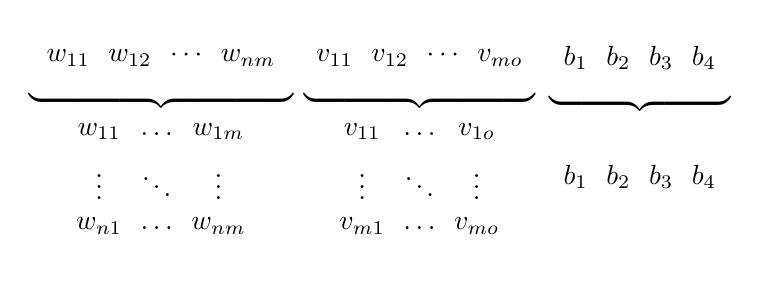
\begin{tikzpicture}
  %% upper nodes
  %\matrix (m1) [upper matrix] {
    %|[box 1=01000000]| sentry &
    %|[box 1=01000001]| 2      &
    %|[box 1=01001001]| 18     &
    %|[box 2=11000000]| sentry &
    %|[box 2=11000001]| 3      &
    %|[box 3=11010000]| sentry &
    %|[box 3=11010001]| 11     &
    %|[box 3=11011001]| 27     \\
  %};
  %% chain
  %\begin{scope}[start chain]
    %\foreach \i in {1, ..., 8} {
      %\chainin (m1-1-\i);
    %}
  %\end{scope}
  %% lower nodes
  \matrix (m1) [upper matrix] {
      w_{11} & w_{12} & \cdots & w_{nm}\\
  };
  \matrix (m2) [right=1pt of m1, upper matrix] {
      v_{11} & v_{12} & \cdots & v_{mo}\\
  };
  \matrix (m3) [right=1pt of m2, upper matrix] {
      b_1 & b_2 & b_3 & b_4 \\
  };
  \matrix (n1) [below=7pt of m1, lower matrix] {
      w_{11} &  \ldots& w_{1m}\\
      \vdots &  \ddots& \vdots\\
      w_{n1} &  \ldots& w_{nm}\\
  };
  \matrix (n2) [below=7pt of m2, lower matrix] {
      v_{11} &  \ldots& v_{1o}\\
      \vdots &  \ddots& \vdots\\
      v_{m1} &  \ldots& v_{mo}\\
  };
  \matrix (n3) [below=21pt of m3, lower matrix] {
      b_1 & b_2 & b_3 & b_4 \\
  };
  %% curving arrows
  %\draw[arrow, looseness=0.6, out=120, in=-50] (m2-1-3.north) to (m1-1-1.south);
  %\draw[arrow, out=90, in=-105] (m2-1-4.north) to (m1-1-4.south);
  %\draw[arrow, looseness=0.8, out=80, in=-115] (m2-1-12.north) to (m1-1-6.south);
\end{tikzpicture}
\end{document}
